به میخ‌های ۱ و ۲ سه کش و به میخ‌های ۳ و ۴ و ۵، چهار کش متصل است. می‌خواهیم ۵ کش را انتخاب کنیم به طوری که به هر یک از میخ‌ها دقیقا ۲ کش انتخاب شده وصل باشد. در این صورت می‌توانیم کش‌های انتخاب نشده را در نظر بگیریم. 
پس باید هر یک از میخ‌های ۱ و ۲ به یک کش انتخاب نشده و هر یک از میخ‌های ۳ و ۴ و ۵ به دو کش انتخاب شده وصل باشند.
شکل حاصل از این میخ‌ها یک مسیر است که میخ ابتدا و انتها ۱ و ۲ و سه میخ وسط ۳و ۴ و ۵ هستند که برای چینش آن‌ها
$3! = 6$
حالت داریم.
\begin{center}
  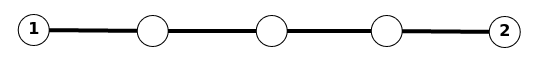
\includegraphics[width=.5\linewidth]{E9_4_2.png}
\end{center}